\chapter{Implementacija i korisničko sučelje}
	\section{Korištene tehnologije i alati}
		Programsko rješenje sastoji se od dva dijela - Android aplikacija i web aplikacija. \\
		
		Android dio pisan je u okruženju AndroidStudio (https://developer.android.com/studio), u nativnom jeziku Java. Za testiranje aplikacije koristili smo ili Android Virtual Device kojeg smo pokretali u okruženju AndroidStudio ili smo aplikaciju direktno instalirali i pokretali na Android uređaju. Baza podataka koju smo koristili za Android je RoomDB koja koristi jezik MySQL. \\
		
		Web dio pisan je u jeziku Python 3, a korišteni framework je Django. Django omogućava lakše razvijanje i upravljanje bazom podataka, funkcijama kao što su login i logout te nudi dinamičko generiranje HTML stranica. Okruženje koje je smo koristili za razvoj serverskog dijela većinom je ovisilo od osobe do osobe. Neki su preferirali Visual Studio Code (https://code.visualstudio.com/), a neki PyCharm (https://www.jetbrains.com/pycharm/), okruženje za Python temeljeno na okruženju IntelliJ. I VSCode i PyCharm nude ugrađene funkcionalnosti za VCS tj. Version Control System. \\
		
		Frontend na web dijelu pisan je u HTML-u uz korištenje bootstrap-a i css-a kako bi aplikacija bila responzivna i za mobilne uređaje i uređaje s velikim zaslonima.
		
		Baza podataka na serverskom dijelu (tj. glavna baza podataka) je Postgres baza podataka. Korišteni SQL jezik je dakle PostgreSQL, a korišteni DB Manager je pgAdmin (https://www.pgadmin.org/). \\
		
		Komunikacija članova tima je realizirana preko aplikacije Slack (https://slack.com/) i Whatsapp, a samim verzijama koda se upravljalo preko sustava git stranici Gitlab (https://about.gitlab.com/). \\
		
		Dokumentacija je pisana u okruženju TexStudio (https://www.texstudio.org/) i u xed-u. \\
		
		
		
		
		\eject
	\section{Ispitivanje programskog rješenja}
		\subsection{Ispitivanje komponenti}
			
			Budući da ja aplikacija napisana za Android uređaje ispitivanje komponenti
			se provodi pomoću razreda AndroidJUnit4 (\url{https://developer.android.com/reference/androidx/test/ext/junit/runners/AndroidJUnit4})
			uz korištenje funkcionalnosti dostupnih u modulu JUnit5 (\url{https://junit.org/junit5/})
			
			Testiraju se razne funkcionalnosti dostupne na android uređaju, među kojima
			vrijedi izdvojiti testiranje dohvata podataka iz baze podataka na uređaju, testiranje prikazivanja
			stavki na popisu, testiranje prikazivanja popisa, testiranje prikazivanja adrese trgovina i testiranje
			prikazivanja proizvoda
			
			Primjeri testiranja:
			
			\begin{figure}[H]
				\centering
				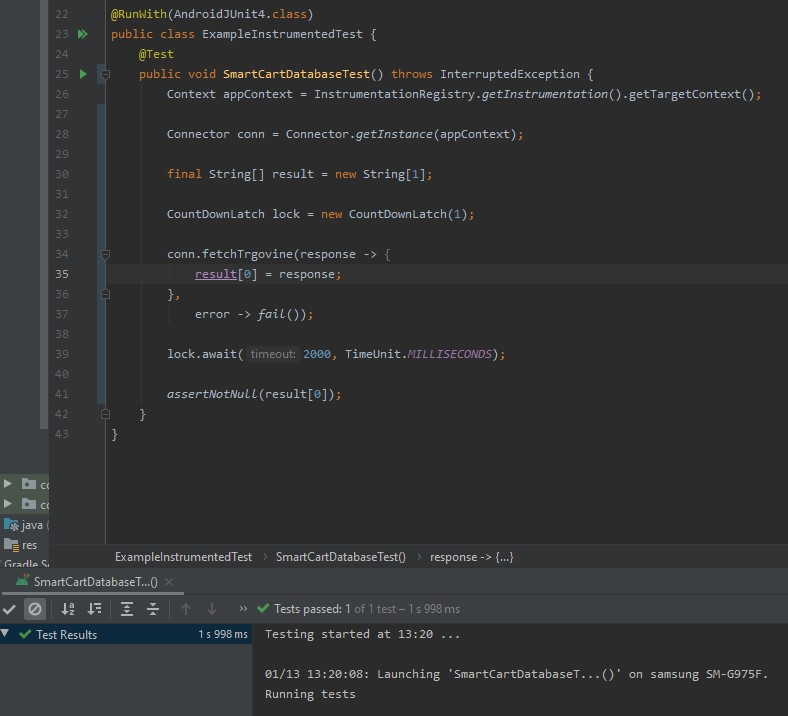
\includegraphics[scale=0.7]{slike/androidTest1.jpg}
				\caption{Testiranje baze podataka na uređaju}
				\label{fig:test_uredaj_db}
			\end{figure}
		
			\begin{figure}[H]
				\centering
				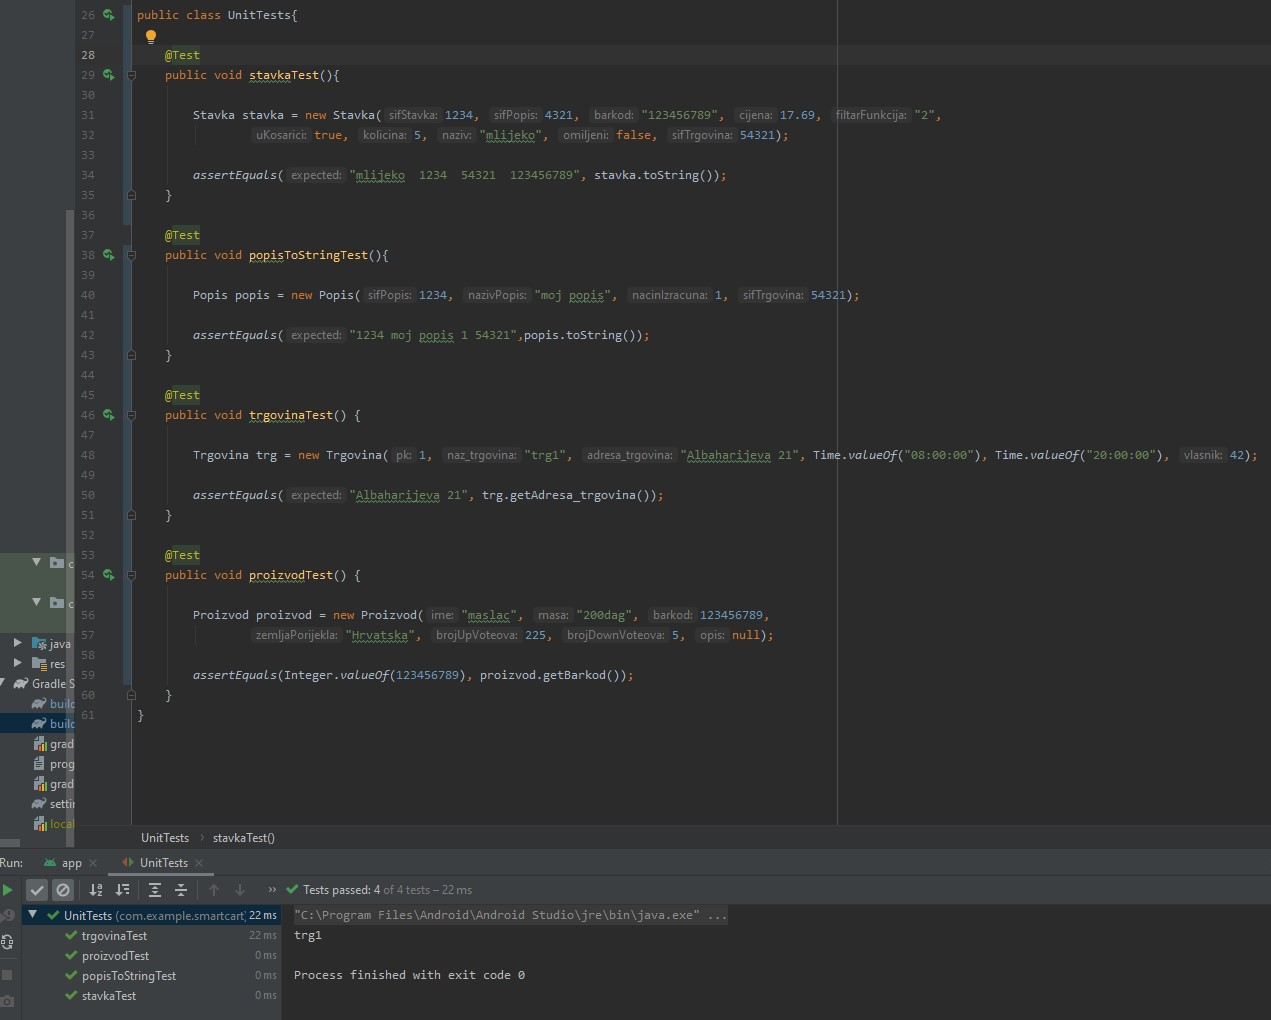
\includegraphics[scale=0.5]{slike/androidTest2.jpg}
				\caption{Testiranje razreda na uređaju}
				\label{fig:test_uredaj_class}
			\end{figure}
		
		\subsection{Ispitivanje sustava}
			
			Ispitivanje sustava je provedeno koristeći funkcionalnosti iz paketa unittest koji dolazi u instalaciji programskog jezika Python u kombinaciji sa alatom Selenium WebDriver koji pruža podršku za automatsko upravljanje internetskim preglednikom. Za instalaciju podrške za ispitivanje sustava potrebno je sa interneta skinuti Selenium za programski jezik Python (\url{https://pypi.org/project/selenium/}, također je moguće instalirati ako se unutar naredbenog retka pozove komanda \textit{pip install selenium}). Uz Selenium za Python potrebno je instalirati i Selenium WebDriver. U našem projektu koristimo geckodriver 0.28.0, verziju Selenium WebDriver-a za internetski preglednik Mozilla Firefox, koja se može skinuti sa sljedeće web-adrese: (\url{https://github.com/mozilla/geckodriver/releases/tag/v0.28.0}).\\
			Nad sustavom se provode razna testiranja. Neka od najvažnijih su:
			
			\begin{itemize}
				\item Testiranje izrade novog profila i pokušaja prijave na web-stranicu pomoću točne i krive kombinacije (relevantan isječak iz koda):
				\lstset{language=Python, tabsize=4, showstringspaces=false, basicstyle=\small}
				\begin{lstlisting}[breaklines]
def fill_login_form(self, username, password):
    self.driver.get(HOME_PAGE)
    self.driver.find_element(By.XPATH, '//button[text()="Log in"]').click()
    self.driver.find_element(By.NAME, "username").send_keys(username)
    self.driver.find_element(By.NAME, "password").send_keys(password)
    self.driver.find_element(By.NAME, "submit_button").click()
					
def test_successful_login(self):
    self.fill_login_form("ante@fer.hr", "pwd")
    self.assertEqual(self.driver.current_url, f"{HOME_PAGE}/trgovac")
					
def test_wrong_login(self):
    self.fill_login_form("ante@fer.hr", "abc")
    self.assertTrue(str(self.driver.current_url).startswith(f"{HOME_PAGE}/login"))
					
def test_create_new_profile(self):
    self.driver.get(HOME_PAGE)
    self.driver.find_element(By.XPATH, '//button[text()="Sign up as kupac"]').click()
    self.driver.find_element(By.NAME, "email").send_keys(NEW_USERNAME)
    self.driver.find_element(By.NAME, "password").send_keys(NEW_PASSWORD)
    self.driver.find_element(By.NAME, "confirm_password").send_keys(NEW_PASSWORD)
    self.driver.find_element(By.NAME, "submit_button").click()
    self.fill_login_form(NEW_USERNAME, NEW_PASSWORD)
    self.assertTrue(f"Logged in as {NEW_USERNAME}" in self.driver.page_source)	
				\end{lstlisting}
				\item Testiranje dodavanja novog proizvoda (relevantan isječak iz koda):
				\begin{lstlisting}[breaklines]
def test_adding_new_barcode(self):
	self.fill_login_form("ante@fer.hr", "pwd")
	self.driver.find_element(By.NAME, "barkod_artikla").send_keys(BARCODE)
	self.driver.find_element(By.NAME, "new_barcode_button").click()
	list_of_products = self.driver.find_element(By.ID, "products")
	self.assertTrue(BARCODE in list_of_products.text)
				\end{lstlisting}
				\item Testiranje „sigurnosti“ stranice (nepostojeći linkovi i pristup linkovima koji zahtjevaju posebnu dozvolu) (relevantan isječak iz koda):
				\begin{lstlisting}[breaklines]
def test_wrong_link(self):
	self.driver.get(f"{HOME_PAGE}/another_link/that_doesnt_exist")
	self.assertEqual(self.driver.current_url, f"{HOME_PAGE}/")

def test_page_permissions(self):
	self.fill_login_form(NEW_USERNAME, NEW_PASSWORD)
	self.driver.get(f"{HOME_PAGE}/trgovac")
	self.assertEqual(self.driver.current_url, f"{HOME_PAGE}/")
				\end{lstlisting}
			\end{itemize}
		
			Razultati testiranja:
			\begin{figure}[H]
				\centering
				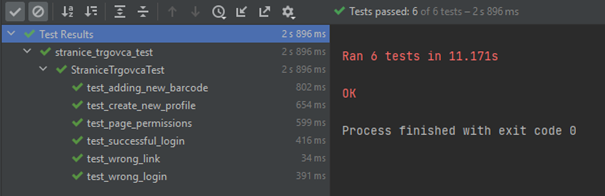
\includegraphics{slike/serverTest.png}
				\caption{Razultati testiranja servera}
				\label{fig:test_server}
			\end{figure}
		\eject
	\section{Dijagram razmještaja}
			Server i serverska baza podataka nalaze se na jednom računalu. Korisnik ima nekoliko opcija ako želi pristupiti aplikaciji. Korisnik može web aplikaciji pristupiti iz bilo kojeg web preglednika. Nadalje, korisnik može aplikaciji pristupiti i preko Android uređaja na kojem je instalirao SmartCart aplikaciju. Android aplikacija, kao i web aplikacija, komunikaciju sa serverom obavljaju HTTP protokolom.
		
			\begin{figure}[H]
				\centering
				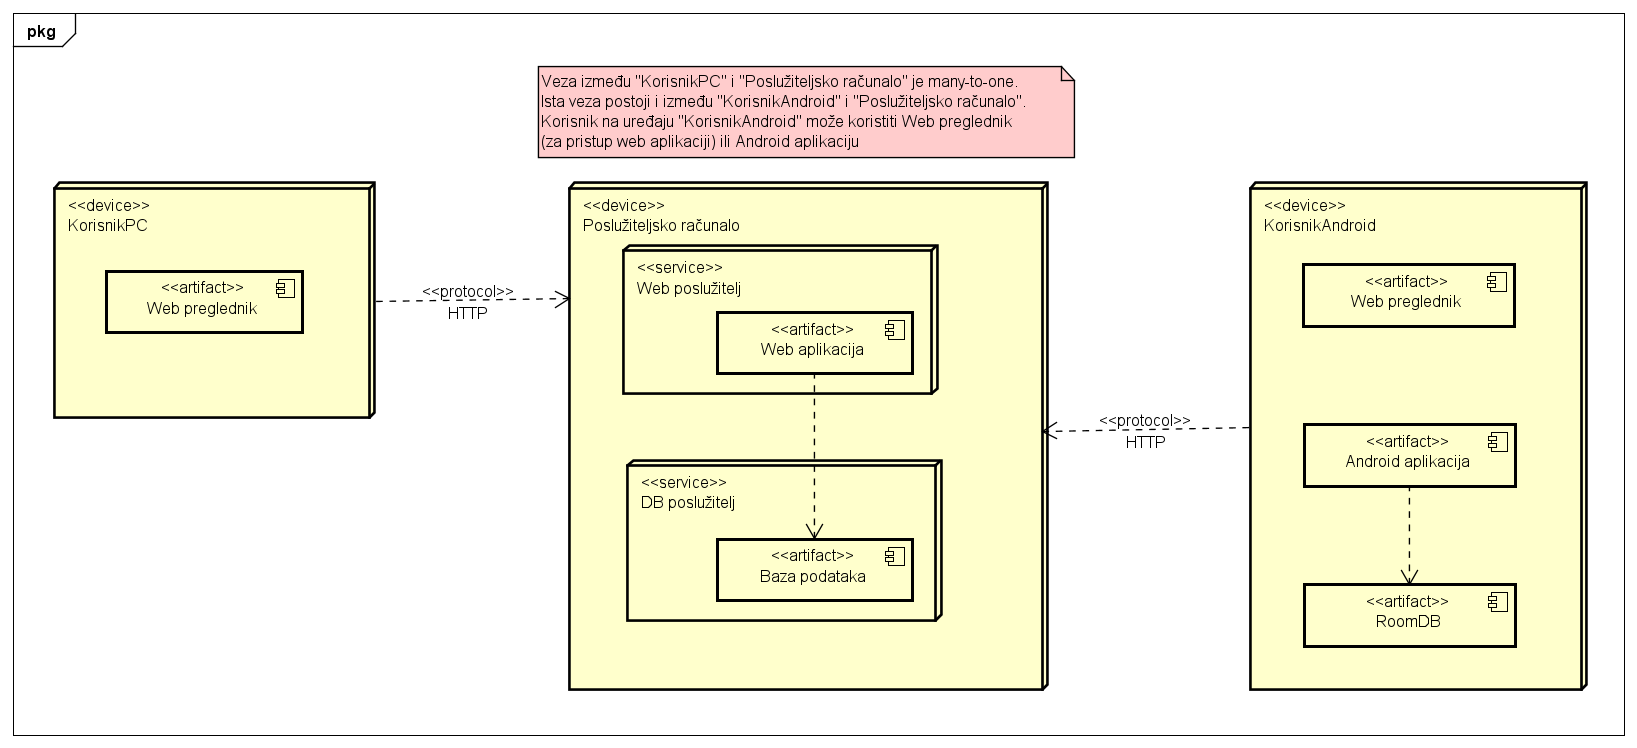
\includegraphics[width=1.0\linewidth]{dijagrami/deployment.png}
				\caption{Dijagram razmještaja}
				\label{fig:deployment}
			\end{figure}
		\eject
	\section{Upute za puštanje u pogon}
		Upute za puštanje u pogon napisane su za linux operacijski sustav.
		Za pokretanje aplikacije na javnom poslužitelju potrebno je napraviti račun za Heroku na stranici \url{https://signup.heroku.com/}.
		Zatim treba instalirati heroku na računalo i ulogirati se naredbama: \\
		\code{sudo snap install --classic heroku}\\
		\code{heroku login}
		\\
		Nakon toga treba se pozicionirati u korijensku mapu repositoryja (preljevstoga) i stvoriti heroku projekt naredbom: \\
		\code{heroku create ime-projekta} \\
		Za stvaranje baze podataka pokrenite \\
		\code{heroku addons:create heroku-postgresql} \\
		Dohvatite url baze podataka i kopirajte ga u varijablu okruženja na Heroku. \\
		\code{heroku pg:info} \\
		\code{heroku config:set DATABASE\_URL=postgres://kopirani/url CREATE\_DB=True FILL\_DB=True} \\
		Zatim je potrebno stvoriti ključ za django aplikaciju naredbom \\
		\code{python3 izvorniKod/backend/generate\_django\_key.py} \\
		Taj ključ spremljen je u datoteci temp u mapi izvorniKod/backend. Spremite ga na Heroku, ali ne kopiranjem, da ne ostane u povijesti terminala nego sljedećom naredbom: \\
		\code{heroku config:set SECRET\_CODE=\$(< izvorniKod/backend/temp)} \\
		Kako biste omogućili Google sign in u Vašoj aplikaciji, stvorite pomoću Vašeg Google računa
		Google ID i ključ za svoj projekt prema uputama u odlomku"Create authorization credentials" na stranici \url{https://developers.google.com/identity/sign-in/web/sign-in}. Google ID zalijepite u red 192 u izvorniKod/backend/settings.py, a gmail adresu tog raučuna 166. red iste datoteke. Tajni ključ kopirajte u neku novu datoteku (npr. umjesto django ključa u izvorniKod/backend/temp. Pošaljite taj ključ na Heroku naredbom: \\
		\code{heroku config:set GOOGLE\_CLIENT\_SECRET=\$(< izvorniKod/backend/temp)} \\
		\textbf{Maknite datoteke s ključevima iz repozitorija!}
		Commitajte promjene i pushajte na Heroku. \\
		\code{git add .} \\
		\code{git commit -m "Promijenjena gmail adresa za slanje poruka"} \\
		\code{git push heroku master} \\
		Na kraju onemogućite stvaranje i punjenje baze podataka jer već sadrži sve što treba. \\
		\code{heroku config:set CREATE\_DB=False FILL\_DB=False} \\
		Ako je sve prošlo kako treba, aplikacija je dostupna na ime-projekta.herokuapp.com.
		\\
		\\
		Za pokretanje aplikacije na mobitelu otvorite izvorniKod/android pomoću Android studija i u klasi Connector izmijenite varijablu host u url vašeg Heroku projekta. Spojite mobitel i pokrenite aplikaciju
		pritiskom na "run".
		
		
		
		\eject
			
